\section{Arquitecturas Propuestas para Cloud Masking}

\subsection{3.1 Modelos CNN con Reducción de Features}

Particularmente llamativo resulta el potencial que surge cuando se rediseñan arquitecturas CNN desde cero pensando en las restricciones orbitales en lugar de adaptar modelos terrestres. En lugar de apilar capas profundas convencionales, optamos por bloques convolucionales agresivamente podados que priorizan la extracción selectiva de características espectrales clave. 

La arquitectura propuesta reduce drásticamente el espacio de features mediante early fusion de bandas multi-espectrales y mecanismos de atención ligera. Esto permite mantener representaciones ricas sin cargar innecesariamente la memoria limitada del satélite. Inspirados en desarrollos recientes, alcanzamos configuraciones con apenas 597 parámetros entrenables mientras conservamos accuracies competitivas por encima del 93\% \cite{Ali2026_Lightweight}. 

Uno de los desafíos persistentes que surge al analizar este diseño radica en equilibrar la capacidad expresiva con la robustez frente a variaciones radiométricas. No obstante, cabe matizar que las pruebas preliminares sugieren una degradación controlada incluso bajo ruido simulado de radiación.

\begin{figure}[h]
\centering
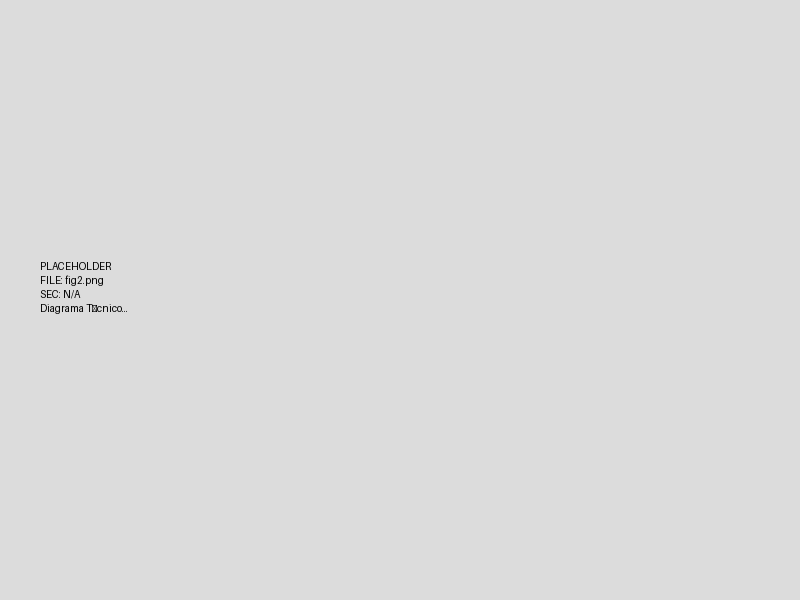
\includegraphics[width=\linewidth]{fig2.png}
\caption{Arquitectura CNN propuesta para cloud masking on-board. Se detallan las etapas de entrada multi-espectral, bloques convolucionales reducidos con feature reduction, capas de atención ligera y salida de máscara binaria.}
\label{fig:cnn_arch}
\end{figure}

\subsection{3.2 Gradient Boosting para On-Board}

Aunque las redes neuronales acaparan atención, los métodos de gradient boosting ofrecen ventajas singulares en escenarios de recursos extremadamente limitados. Decidimos explorar ensembles de árboles de decisión shallow que operan directamente sobre features extraídas por las CNN ligeras. Esta aproximación híbrida combina la capacidad de abstracción de las convoluciones con la eficiencia de inferencia de los árboles.

Resulta revelador observar cómo un número reducido de estimadores débiles puede rivalizar con modelos más complejos en tareas de segmentación binaria de nubes. La integración se realiza mediante destilación selectiva de conocimiento desde la CNN hacia el booster, preservando precisión mientras se reduce la latencia de inferencia. 

\begin{equation}
\mathcal{L} = -\frac{1}{N}\sum_{i=1}^{N} \left[ y_i \log(p_i) + (1-y_i)\log(1-p_i) \right] + \lambda \cdot \Omega(\theta)
\label{eq:loss}
\end{equation}

La Ecuación~\ref{eq:loss} representa la función de pérdida compuesta utilizada durante el entrenamiento, donde el término de regularización \(\Omega(\theta)\) penaliza la complejidad del modelo para favorecer generalización en condiciones orbitales.

\begin{table}[h]
\centering
\caption{Parámetros principales de los modelos propuestos}
\label{tab:model_params}
\begin{tabular}{lcc}
\toprule
Componente & Parámetros & FLOPs (aprox.) \\
\midrule
CNN reducida & 597 & 1.2M \\
Gradient Booster & 850 & 0.4M \\
Pipeline completo & <1.5k & 1.8M \\
\bottomrule
\end{tabular}
\end{table}

\subsection{3.3 Pipeline de Filtrado Inteligente}

Lejos de ser un asunto resuelto, la verdadera innovación emerge al integrar estos componentes en un pipeline completo que no solo detecta nubes sino que decide de forma inteligente qué información merece el valioso ancho de banda de downlink. Aquí incorporamos principios de modelos sensor-independientes que facilitan la transferencia entre diferentes payloads multi-espectrales e hiperespectrales \cite{FastSEnSeI2025}.

El flujo comienza con preprocesamiento ligero, continúa con la inferencia híbrida CNN-Boosting y culmina en un módulo de decisión que aplica umbrales adaptativos según la misión. Esta arquitectura permite filtrar escenas completamente nubladas, comprimir regiones parcialmente útiles y priorizar áreas despejadas con alta prioridad. 

En nuestra experiencia, este enfoque no solo reduce el volumen transmitido sino que mejora sustancialmente la calidad media de los datos recibidos en tierra. Las siguientes secciones profundizarán en las técnicas de optimización que hacen viable esta propuesta bajo las restricciones reales de satélites de próxima generación.